\documentclass[border=4pt]{standalone}
\usepackage{tikz}
\usetikzlibrary{arrows,arrows.spaced}
\begin{document}
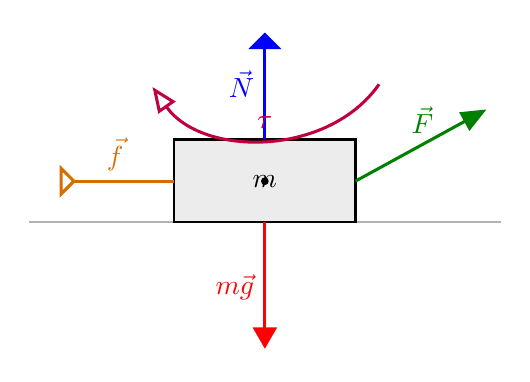
\begin{tikzpicture}[force/.style={line width=1.1pt}]
  \draw[gray!60,line width=.7pt] (-3,0) -- (3,0);
  \draw[fill=gray!15,line width=.8pt] (-1.15,0) rectangle (1.15,1.05);
  \node at (0,.52) {$m$};

  \draw[force,blue,-{spaced triangle 90}] (0,1.05) -- node[left] {$\vec N$} (0,2.45);
  \draw[force,red,-{spaced triangle 60}] (0,0) -- node[left] {$m\vec g$} (0,-1.65);
  \draw[force,green!50!black,-{spaced triangle 45}] (1.15,.52) -- node[above] {$\vec F$} (2.85,1.45);
  \draw[force,orange!85!black,-{spaced open triangle 90 reversed}]
    (-1.15,.52) -- node[above] {$\vec f$} (-2.65,.52);
  \draw[force,purple,-{spaced open triangle 45}]
    (1.45,1.75) to[bend left=55] node[above,sloped] {$\tau$} (-1.45,1.75);
  \fill (0,.52) circle (1.4pt);
\end{tikzpicture}
\end{document}
